\subsection{Моделиране}

\subsubsection{Моделиране на тяга от витло и мотор}

За моделиране на моторът и витлото е приет опростеният модел:
Който моделира системата, коефициент на усливане и нискочестотен филтър.

\begin{figure}[htpb!]
    \centering
    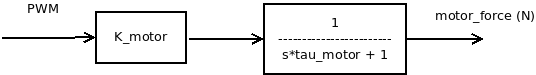
\includegraphics[width=0.7\textwidth]{motor_model}
    \caption{Опростен модел на витло и мотор}
    \label{fig:motor_model}
\end{figure}

\begin{equation}
    G_{motor}(s) = \frac{k_{motor}}{s \tau_{motor} + 1}
    \label{eqn:motor_model}
\end{equation}

Реално този модел не е добра апроксимация на тягата на моторите,
защото реалната характеристика е нелинейна и се променя спрямо множество параметри (напрежение на батерията, температура, налягане, вляжност, скорост),
но за неголеми времеви интервали и неголеми промени в входният сигнал статичната характеристика
може да бъде описана достатъчно добре, чрез линейната апроксимация (\autoref{eqn:motor_model}).


\subsubsection{Моделиране на платформа за управление на ъгъл на завъртане}

За моделиране на платформата за управление на ъгъл на завъртане (\autoref{fig:balance_force_diagram})
нека приемем, че въртящата час е пренебрежимо тънка, с дължина \(l\), и има маса \(M\). 
Ъгълът, който въртящата част сключва с хоризонта е означен с \(\phi\).
Във края на рамената се намират безчетковите мотори и витлата, моделирани, като концентрирани
маси с големина \(m\), като всеки от тях има сила на тягата означена с \(F_1, F_2\) респективно.
Триенето с въртящата ос е моделирано с коефициентът на триене \(C\).

\begin{figure}[htpb!]
    \centering
    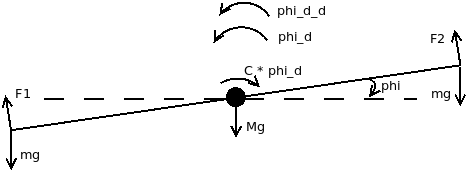
\includegraphics[width=0.7\textwidth]{balance_force_diagram}
    \caption{Диаграма на платформа за управление на ъгъл на завъртане}
    \label{fig:balance_force_diagram}
\end{figure}

От втори закон на Нютон \autoref{eqn:newton1}, 
\begin{equation}
    I \ddot{\phi} = \sum_i \tau_i
    \label{eqn:newton1}
\end{equation}
От където следва:
\begin{equation}
    I \ddot{\phi} = F_2*\frac{l}{2} - F_1*\frac{l}{2} - C \dot{\phi}
    \label{eqn:newton1_expand}
\end{equation}
Нека:
\begin{equation}
    F_2 = F_0 + \delta f, F_1 = F_0 - \delta f 
\end{equation}
След като заместим в \autoref{eqn:newton1_expand}
\begin{equation}
    I \ddot{\phi} = (F_0 + \delta f)*\frac{l}{2} - (F_0 - \delta f)*\frac{l}{2} - C \dot{\phi}
\end{equation}
Плучаваме:
\begin{equation}
    I \ddot{\phi} + C \dot{\phi} = l * \delta f
\end{equation}
Което опростява системата до линейна SISO система.

Апроксимираме инерционният момент \(I\) като :
\begin{align}
    I &= I_{rod} + 2*I_{motor}\\
    I &= \frac{1}{12}Ml^2 + 2m(\frac{l}{2})^2 \\
    I &= \frac{l^2}{12}(M + 6m)
\end{align}

При нулеви начални условия след трансформация на Лаплас получаваме:
\begin{equation}
    s^2 I \bar{\Phi}(s) + s C \bar{\Phi}(s) = l * \bar{\delta f}(s) 
\end{equation}
От където получаваме предавателната функция:
\begin{equation}
    G_{platform}(s) = \frac{\bar{\Phi}(s)}{\bar{\delta f }(s)} = \frac{l}{s ( s I + C)}
\end{equation}

За получаване на предавателната функция на отворената система:
\begin{equation}
    G_{sys} = G_{motor}(s)G_{platform}(s) = 
    \frac{k_{motor} l}{s( s I + C)(s \tau_{motor} + 1)} 
\end{equation}


\subsubsection{Моделиране на платформа с 4 ротора}

\FloatBarrier
Безполитните летателни платформи с 4 ротора се разделят на 2 основни дизайна "+" и "х". 
Х-конфигурацията се счита за по-стабилна, от колкото + конфигурацята.

Рамката на платформата се състои от 2 кръстосани рамена, като роторите са монтирани в краищата им.
Роторите на всяко рамо се въртят в противоположни посоки както е показано на фигура\ref{fig:rotors}
Важно е да се отбележи, че перките на ротори 1 и 3 имат обратен наклон  спрямо перките на роторите 2 и 4.
Така тягата на всияки ротори е в еднаква посока. Респективно различната посока на въртене на роторите е нужна
за да може приведеният въртящ момент да бъде равен на нула, за да може платформата да запазва своята ориентация.

\begin{figure}[!h]
	\centering
	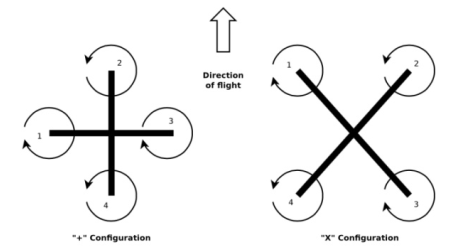
\includegraphics[width=0.6\columnwidth]{rotors}
	\caption{Основни типове на конфигурация .}
	\label{fig:rotors}
\end{figure}


Тук е важно да дефинираме 2 основни координатни системи, които ще използваме. 
Първата е спрямо земята (XE,YE,ZE)  а втората е спрямо тялото на квадракоптера (XB,YB,ZB).
Ориентацията на квадракоптера може да се дефинира чрез Ойлеровите ъгли на тялото на квадракоптера.
На фигура\ref{fig:kinematika} са показани коростите на въртене на роторите \( \omega_1 , \omega_2 ,
\omega_3 , \omega_4 \), силите на тягата генерирана от перките \(T_1,T_2,T_3,T_4\).

Позицията на квадракоптера е дефинирана, в координатната система спрямо земята по осите x,y,z с вектора 
\(\xi = [x,y,z]^T\). А ориентацията се дава, чрез Ойлеровите ъгли \(\eta = [\phi,\theta,\psi]^T\).
А векторът \(q = [\xi,\eta]^T\) съдържа както се вижа и линейлите и ъгловите кооргинати.

Центъра на масите на дрона се смята за основа на координатната система на тялото на дрона. Спямо тялото на дрона
линейните скорости се определят от \(JB = \begin{bmatrix}Jx,B\\Jy,B\\Jz,B\end{bmatrix}\) а ъгловите скорости се
определят от \(\omega = \begin{bmatrix}p\\q\\r \end{bmatrix}\)

\begin{figure}[!h]
    \centering
    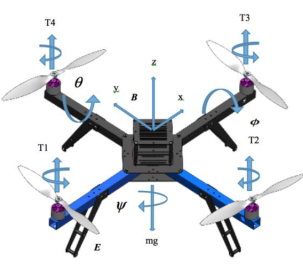
\includegraphics[width=0.6\columnwidth]{kinematika}
    \caption{Сили, моменти и отправни системи на квадракоптера}
    \label{fig:kinematika}
\end{figure}

За да може квадракоптерът да се носи във въздуха е нужно да са спазени следните условия:

\begin{align}
		\sum_{i=1}^{4} T_i  =& -mg \\
		\sum_{i=1}^{4} M_i  =& 0 \\
		T_{1,2,3,4} ||& g \\
		( \omega_1 + \omega_3 ) - ( \omega_2 + \omega_4 ) =& 0 
\end{align}

от което и следва, че \(\phi=0,\theta=0,\psi=0\).

При увеличаване/намаляване на скоростта на роторите дронът може да се движи, нагоре и надолу.
За да се движим нагоре : \(\sum_{i=1}^4 T_i > -mg\).
И респективно да се двиим надолу: \(\sum_{i=1}^4 T_i < -mg\). Като не забравяме, 
че и в двата случая другите параметри остават незасегнати.

За промяна на ориентацията се налага да:
\begin{align}
		\dot{\psi} = k_{\psi}((\omega_1+\omega_3)-(\omega_2 + \omega_4)) ,& \psi = \int \dot{\psi}dt\\
		\dot{\phi} = k_{\phi}((\omega_1 + \omega_4) - (\omega_2+\omega_3 )) ,& \phi = \int \dot{\phi}dt\\
		\dot{\theta} = k_{\theta}((\omega_1+\omega_2) - (\omega_3 +\omega_4)) ,& \theta = \int \dot{\theta}dt
\end{align}


От което следва, че при намаляне на скоростта на ротор 2 и уваличаване на скоростта на ротор 4 постигаме
завъртане по \(\phi\). Съответно намаляване на скоростта на ротор 1 и увеличаване на скоростта на ротор 3 
постигаме завъртане по \(\theta\)  и съответно намаляване на скоростта на срещуположни ротори и съотетно увеличаване на другите два посигаме завъртане по \(\psi\).

\begin{figure}[!h]
    \centering
    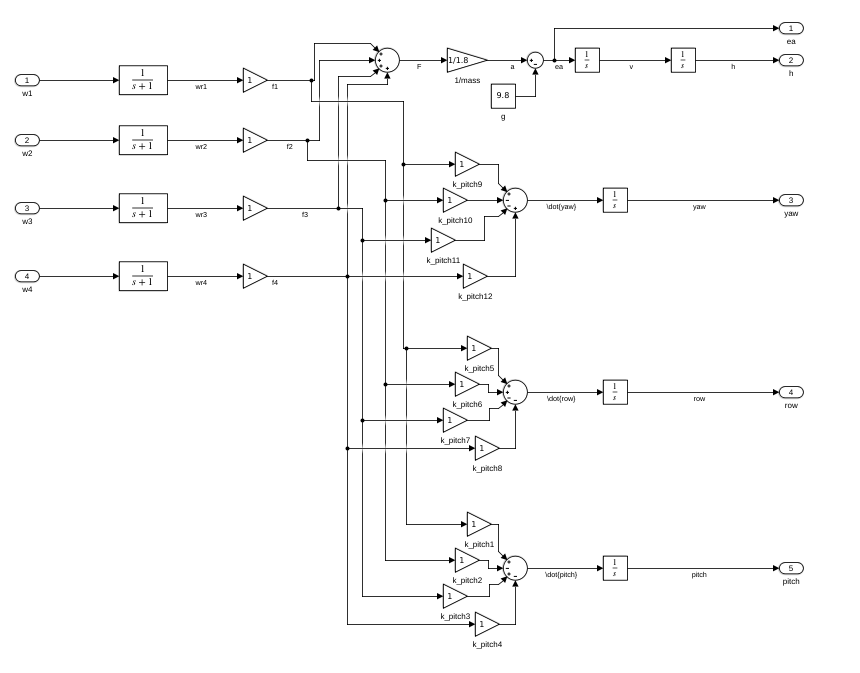
\includegraphics[width=0.8\columnwidth]{quadrotor_simulink}
    \caption{SIMULINK схема на динамиката на платформа с 4 ротора.}
    \label{fig:quadrotor_simulink}
\end{figure}


\FloatBarrier


\subsection{Компенсация на сензорни отмествания}

\subsubsection{Компенсация на жироскопен дрейф}
\FloatBarrier
Жироскопите обикновено не са силно зашумени за разлика от
акселерометрите, но имат своите недсостатъци.
Основен проблем при жироскопите е т.нар. жироскопен дрейф.
В неподвижно състояние жироскопът показва малко постоянно завъртане в някоя посока.
Жироскопният дрейф зависи основно от температурата.

За да калибрираме и занулим стойностите на жироскопа
се налага да направим полиномиална компенсация по температура.

За целта жироскопа е ухладен до \(0^{\circ}C\)
след което е поставен неподвижно бавно да се загрее в продължение на 45мин до стайна температура.
През цялото време събираме данните от жироскопа и измерената от бордовия термометър температура.
След приключване на експеримента използваме матлаб за намиране на полином,
който точно описва получените данни за всяка от осите.

\begin{figure}[htpb!]
    \centering
    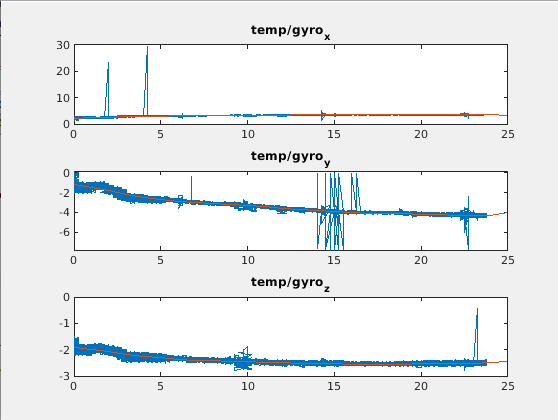
\includegraphics[width=0.9\textwidth]{gyro_drift_calibrate}
    \caption{Жироскопен дрейф спрямо температура и полиномиална компенсация спрямо температура}
    \label{fig:gyro_drift_calibrate}
\end{figure}

\begin{lstlisting}[language=matlab, caption={Получени полиноми за коменсация на жироскопният дрейф}, label={lst:gyro_drift_poly}]

    p_x =

     -42.6978e-9  3.7797e-6  -131.8066e-006  2.2717e-3  -19.5918e-3  67.9744e-3  95.1384e-3  2.2440e+0

  p_y =
  
      87.1716e-9  -7.6384e-6  263.1019e-006  -4.4660e-3  37.8030e-3  -129.2365e-3  -191.6577e-3  -1.1695e+0
  p_z =
  
      15.9591e-9  -1.4613e-6  53.0721e-006  -961.5439e-6  8.8365e-3  -33.3197e-3  -44.0584e-003  -1.9076e+0

\end{lstlisting}


\FloatBarrier


\subsubsection{Компенсация на магнитни отмествания от околната среда}
\FloatBarrier
Магнитометрите имат постоянно отместване поради средата в която се намират.
Това отместване се дължи на металните и магнитни обекти,
както и всички електромагнитни смущения причинени от заобикалящата ни среда.
Поради факта, че в близката ни околна среда тези смущения са постоянни, което означава, че ние можем да ги компенсираме статично.


За целта поставяме сензора в нормална позиция и бавно го завъртаме, като се стараем да покрием възможно най-много ъглови комбинации.
След получаване на данните виждаме, че те образуват Елипсоид с отместен център.
Използваме техника на Мерайо.
Идентифицираме елипсоида и отместването на центъра,
след което правим трансформация елипсоид-сфера,
след което изваждаме отместването на центъра.
Верифицираме резултатът, като виждаме, че всички измерени точки са в допостим диапазон от повърхността на сфера с център 0 и радиус 1.

\begin{figure}[htpb!]
    \centering
    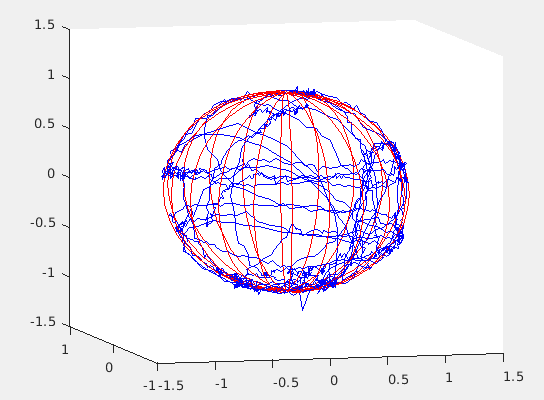
\includegraphics[width=0.9\textwidth]{mag_calibration}
    \caption{Компенсирани данни получени от магнитометър}
    \label{fig:mag_calibration}
\end{figure}

\begin{lstlisting}[language=matlab, caption={Получени трансформация елипсоид-сфера и отместване на център}, label={lst:mag_cal_trans}]

    U =

    21.4229e+000   837.9000e-003     3.0861e+000
     0.0000e+000    21.6201e+000     2.0207e+000
     0.0000e+000     0.0000e+000    27.2441e+000

    c =

    -1.6000e-003
    19.9000e-003
    45.7000e-003

\end{lstlisting}


\subsection{Калманов наблюдаел}

Калмановият наблюдател е рекурсивен естиматор на 
състоянието на системата, който дава статистически
оптимална естимация на състоянието дори и при използване на
зашумени входни данни.
Калмановият филтър често се използва при т.нар сензорно сливане,
и е най-честият метод, който се използва 
за обединяване на жироскоп и акселерометър за намиране на ориентация.
Калмановият филтър може да бъде разделен на 2 основни стъпки: предсказване и обновяване.

В стъпка предсказване алгоритъма продуцира оценка за състоянието, както и за неопределеностите в състоянието,
в резултат на шум. Тази стъпка може да бъде изпълнена множество пъти, като предсказанието е все по-неопределеност с всяка итерация.
В стъпка обновяване алгоритъма сравнява предсказанията спрямо зашумените измервания и обновява
оценката използвайки претеглена комбинация 
от предсказание и измерване, като се дава по-високо
тегло на оценкитв с по-ниска неопределеност.

Алгоритъма може да бъде изпълняван на всяка итерация,
без нужда от стари стойности на използваните променливи.

Крайната естимация може да бъде описана като оптимално решение,
коато системата е линейна и е зашумента от шум в състоянията и шумове от измерванията с Бял Гаусов Шум.
Можем да представим това математически чрез модел на предсказанието 
и модел на измерването.

\begin{align}
    x_k = F x_{k-1} + B u_k + N(0, Q_k) \\
    z_k = H x + N(0, R_k)
\end{align}

Филтърът ще бъде използван за оценка на ойлеровите ъгли, на завъртане спрямо оста X и оста Y.
Така дефинираме вектор на състоянията във форма:
\begin{equation*}
    x = 
    \begin{bmatrix}
        \phi\\
        \psi\\
        \omega_{xb}\\
        \omega_{yb}
    \end{bmatrix}_k
\end{equation*}

Моделите на измерване и предсказване са дефинирани:
\begin{align}
    \begin{bmatrix}
        \phi\\
        \psi\\
        \omega_{xb}\\
        \omega_{yb}
    \end{bmatrix}_k &=
    \begin{bmatrix}
        1 & 0 & -d_t & 0 \\
        0 & 1 & 0 & -d_t \\
        0 & 0 & 1 & 0 \\
        0 & 0 & 0 & 1
    \end{bmatrix}_k *
    \begin{bmatrix}
        \phi\\
        \psi\\
        \omega_{xb}\\
        \omega_{yb}\\
    \end{bmatrix}_{k-1}
    +
    \begin{bmatrix}
        d_t & 0 & 0 & 0 \\
        0 & d_t & 0 & 0 \\
        0 & 0 & 0 & 0   \\
        0 & 0 & 0 & 0
    \end{bmatrix}_k *
    \begin{bmatrix}
        \omega_{x}\\
        \omega_{y}\\
        0 \\
        0
    \end{bmatrix}_{k}
    +
    N(0, Q_k) \\
    \begin{bmatrix}
        A_\phi\\
        A_\psi\\
        0\\
        0
    \end{bmatrix}_k &=
    \begin{bmatrix}
        1 & 0 & 0 & 0 \\
        0 & 1 & 0 & 0 \\
        0 & 0 & 0 & 0 \\
        0 & 0 & 0 & 0
    \end{bmatrix}_k *
    \begin{bmatrix}
        \phi\\
        \psi\\
        \omega_{xb}\\
        \omega_{yb}\\
    \end{bmatrix}_{k}
    +
    N(0,R_k)
\end{align}

След снемане на експериментални данни са под брани следните
ковариантни матрици:

\begin{align}
    Q =
    \begin{bmatrix}
        33.8 & 0 & 0 & 0 \\
        0 & 33.8 & 0 & 0 \\
        0 & 0 & 0.4 & 0 \\
        0 & 0 & 0 & 0.4
    \end{bmatrix} &,&
    R = \begin{bmatrix}
        32 & 0 & 0 & 0 \\
        0 & 32 & 0 & 0 \\
        0 & 0 & 0 & 0 \\
        0 & 0 & 0 & 0
    \end{bmatrix}
\end{align}

Така синтезирания филтър на Калман е имплемнтиран в контролера.
За проверка на филтъра е изпълнен следният експеримент.
След стартиране изчакваме, за да сме сигурни, че филтърът се е устнановил.
След което накланяме ръчно дрона под ъгъл около \(20^{\circ}\), 
като задържаме ъгъла за няколко секунди поставяме в 
изходно положение отново за няколко секунди,
след което повтаряме наклона в обратната посока и отново задържаме.
Връщаме в изходна позиция изчакваме, след което внасяме допълнителни смущения в системата,
чрез относително силни почувкания в успореднин на на осите на въртене.

Резултатите от експеримента могат да бъдат проверени в (\autoref{fig:kalman_filter_time_vs_raw}, \autoref{fig:kalman_filter_time_vs_raw2})

\begin{figure}[htpb!]
    \centering
    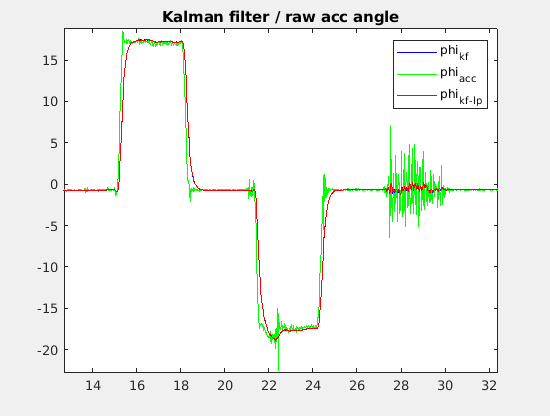
\includegraphics[width=0.8\textwidth]{kalman_filter_time_vs_raw}
    \caption{Проверка на Калман филтъра за ос \(\phi\)}
    \label{fig:kalman_filter_time_vs_raw}
\end{figure}

\begin{figure}[htpb!]
    \centering
    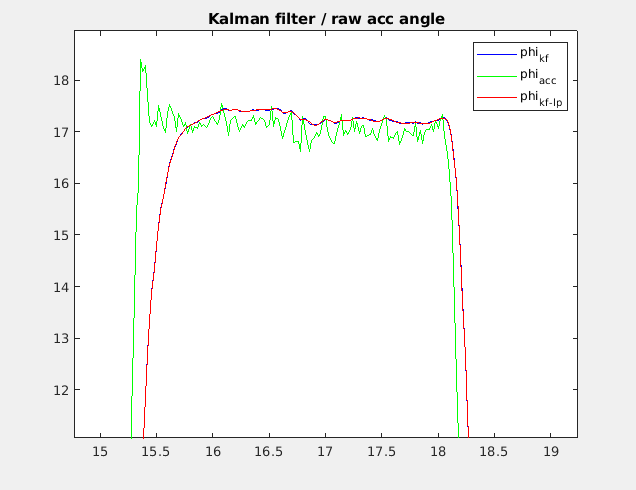
\includegraphics[width=0.8\textwidth]{kalman_filter_time_vs_raw_2}
    \caption{Проверка на Калман филтъра за ос \(\phi\), приближен}
    \label{fig:kalman_filter_time_vs_raw2}
\end{figure}

Забелязваме, че филтъра успешно потиска смущенията и крайният резултат се установява за около \(0.1s\).

\FloatBarrier

\subsection{Експериментални задачи}

\subsubsection{Снемане на статичните характеристики за тягата на мотор с витло}

Характеристиките са снети при използване на напълно заредена батерия.
Процедурата по снемане е както следва:
Използвана е платформата за управление на ъгъл на завъртане,
като под рамо едно е поставена везна. Върху везната се поставя право парче дърво, което да се допира във въртящата част на платформата,
на разстояние от центъра равно на разстоянието на срещуположният двигател от центъра. 
По този начин предаването на сила е 1:1.
Кантара се занулява и се задават управляващи сигнали в диапазона \(950 \to 1950ms\) запълване,
на ШИМ \(50Hz\). при подаването на всеки сигнал се изчаква преходните процеси да преминат и се снема стойността от везната.

\begin{figure}[htpb!]
    \centering
    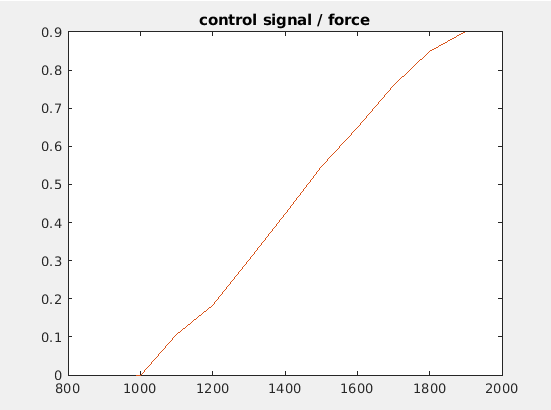
\includegraphics[width=0.7\textwidth]{control_force}
    \caption{Управляващ сигнал / тяга}
    \label{fig:control_force}
\end{figure}

След снемане на характеристиките е изчкислен предавателен коефициент \(k_{motor=1.21e-3}\) в диапазона на управление (\(1300\to1700\)).
Важно е, че характеристиката е почти линейна в диапазона на управление.








